\documentclass[aspectratio=169, table, 12pt]{beamer}

\usepackage{colortbl}
\usepackage{xcolor}
\usepackage{listings}
\usepackage{tabularx}
\usepackage{tikz}
\usetikzlibrary{arrows.meta, positioning, calc, fit, shapes.geometric}

\makeatletter
\def\input@path{{../theme/}}
\makeatother
\graphicspath{{../theme/}{../../figures/}}
\usetheme{Pradita}

\definecolor{praditagreen}{RGB}{37, 113, 71}

% Tema membuat garis tabel berwarna putih. Dikembalikan agar tabel terbaca.
\arrayrulecolor{black}
\setlength{\arrayrulewidth}{0.5pt}

% Menempatkan gambar di tengah kolom, mendatar sekaligus tegak. Lebarnya
% dipenuhi selebar kolom. Bila hasilnya melebihi tinggi yang disediakan,
% tingginya yang menjadi pembatas, sehingga gambar tidak menembus bingkai.
\newsavebox{\kotakkolom}
\newcommand{\gambarkolom}[2][0.72\textheight]{%
  \sbox{\kotakkolom}{\resizebox{\linewidth}{!}{#2}}%
  \begin{minipage}[c][#1][c]{\linewidth}%
    \centering
    \ifdim\dimexpr\ht\kotakkolom+\dp\kotakkolom\relax>#1\relax
      \resizebox{!}{#1}{#2}%
    \else
      \usebox{\kotakkolom}%
    \fi
  \end{minipage}%
}

\lstdefinestyle{PythonStyle}{
  language=Python,
  basicstyle=\ttfamily\scriptsize,
  keywordstyle=\color{blue}\bfseries,
  commentstyle=\color{gray}\itshape,
  stringstyle=\color{red},
  breaklines=true,
  frame=lines,
  backgroundcolor=\color{lightgray!10},
  tabsize=2,
  showstringspaces=false
}

\lstdefinelanguage{bash}{
  keywords={},
  basicstyle=\ttfamily\scriptsize,
  ndkeywords={cd, python, bash, source},
  ndkeywordstyle=\color{purple}\bfseries,
  sensitive=true,
  commentstyle=\color{gray},
  breaklines=true,
  frame=lines,
  backgroundcolor=\color{lightgray!10},
  tabsize=2,
  comment=[l]{\#},
  showstringspaces=false
}

\title{\Huge{CQRS dan Event Sourcing}}
\subtitle{IF231303 Arsitektur Perangkat Lunak}
\author{Alfa Yohannis}

\begin{document}

\frame{\titlepage}

\begin{frame}{{\Large Tujuan Pembelajaran}}
  \vspace{10pt}
  \begin{enumerate}
    \item Menjelaskan pemisahan sisi perintah dari sisi kueri beserta proyeksi
          yang menjembatani keduanya.
    \item Membedakan penyimpanan keadaan sekarang dari penyimpanan event,
          lalu menentukan kapan masing-masing layak dipilih.
    \item Mengukur \textit{write cost} dan \textit{read cost} ketiga versi,
          \textit{replay cost} terhadap panjang \textit{event log}, dan jumlah
          \textit{temporal query} yang terjawab.
  \end{enumerate}

  \vspace{10pt}
  {\small Contohnya buku besar saldo dompet mahasiswa, ditulis tiga kali dengan
  perilaku luar yang sama persis.}
\end{frame}

\begin{frame}{{\Large Pendahuluan}}
  \vspace{8pt}
  \begin{itemize}\small
    \item Bab sebelumnya memakai satu model data untuk menulis sekaligus
          membaca, yaitu bentuk CRUD.
    \item Perintah menuntut keadaan terakhir beserta aturan bisnisnya, sedangkan
          kueri menuntut bentuk yang siap ditampilkan.
    \item CQRS memisahkan model tulis dari model baca. \textit{Event sourcing}
          menyimpan event, bukan keadaan.
  \end{itemize}

  \vspace{8pt}
  {\small Domainnya dompet mahasiswa dengan dua perintah saja, yaitu setor dan
  bayar. Saldonya tidak boleh minus, dan aturan itu diperiksa sisi perintah.}
\end{frame}

\begin{frame}{{\Large Satu Model Dibanding Dua Model}}
  \vspace{10pt}
  \centering
  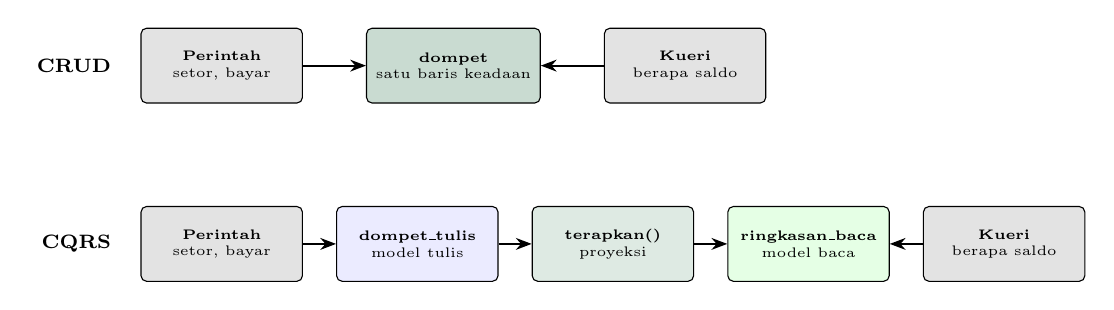
\begin{tikzpicture}[
    kotak/.style={draw, rounded corners=2pt, minimum width=2.05cm,
      minimum height=0.95cm, align=center, font=\tiny\bfseries},
    panah/.style={-{Stealth[length=2mm]}, thick}
  ]
    \node[kotak, fill=gray!22] (kirim1) {Perintah\\
      {\tiny\mdseries setor, bayar}};
    \node[kotak, fill=praditagreen!25, right=0.8cm of kirim1] (tabel1)
      {dompet\\{\tiny\mdseries satu baris keadaan}};
    \node[kotak, fill=gray!22, right=0.8cm of tabel1] (baca1) {Kueri\\
      {\tiny\mdseries berapa saldo}};
    \node[left=0.25cm of kirim1, font=\scriptsize\bfseries] {CRUD};

    \node[kotak, fill=gray!22, below=1.3cm of kirim1] (kirim2) {Perintah\\
      {\tiny\mdseries setor, bayar}};
    \node[kotak, fill=blue!8, right=0.42cm of kirim2] (tulis)
      {dompet\_tulis\\{\tiny\mdseries model tulis}};
    \node[kotak, fill=praditagreen!15, right=0.42cm of tulis] (proyeksi)
      {terapkan()\\{\tiny\mdseries proyeksi}};
    \node[kotak, fill=green!10, right=0.42cm of proyeksi] (bacamodel)
      {ringkasan\_baca\\{\tiny\mdseries model baca}};
    \node[kotak, fill=gray!22, right=0.42cm of bacamodel] (baca2) {Kueri\\
      {\tiny\mdseries berapa saldo}};
    \node[left=0.25cm of kirim2, font=\scriptsize\bfseries] {CQRS};

    \draw[panah] (kirim1) -- (tabel1);
    \draw[panah] (baca1) -- (tabel1);
    \draw[panah] (kirim2) -- (tulis);
    \draw[panah] (tulis) -- (proyeksi);
    \draw[panah] (proyeksi) -- (bacamodel);
    \draw[panah] (baca2) -- (bacamodel);
  \end{tikzpicture}

  \vspace{8pt}
  {\small Pada susunan bawah, kueri berhenti di model baca, dan bentuk model
  baca itu bebas mengikuti pertanyaannya.}
\end{frame}

\begin{frame}{{\Large Tanggung Jawab Ketiga Bagian}}
  \vspace{8pt}
  \centering
  \small
  \begin{tabularx}{0.95\textwidth}{|l|X|X|}
    \hline
    \textbf{Bagian} & \textbf{Tanggung jawab} & \textbf{Tidak boleh mengerjakan} \\
    \hline
    Sisi perintah & Memeriksa aturan bisnis lalu menyimpan perubahannya & Menyusun bentuk tampilan, dan melayani kueri \\
    \hline
    Proyeksi & Melipat perubahan yang diterima ke atas model baca & Menolak perubahan, sebab perubahannya sudah terjadi \\
    \hline
    Sisi kueri & Membaca model baca lalu menyerahkannya apa adanya & Menyentuh model tulis, dan mengubah nilai apa pun \\
    \hline
  \end{tabularx}

  \vspace{8pt}
  {\small Dua konsekuensinya: bentuk model baca bebas mengikuti pertanyaan, dan
  model baca dapat tertinggal dari model tulis.}
\end{frame}

\begin{frame}[fragile]{{\Large Satu Perintah Menulis Dua Kali}}
  \vspace{4pt}
\begin{lstlisting}[style=PythonStyle]
saldo_lama = baris[0] if baris else 0
saldo_baru = domain.periksa_perintah(saldo_lama, perintah)
self.koneksi.execute(
  "INSERT INTO dompet_tulis (pemilik, saldo) VALUES (?, ?) "
  "ON CONFLICT(pemilik) DO UPDATE SET saldo = excluded.saldo",
  (perintah.pemilik, saldo_baru),
)
self.koneksi.commit()
if self.proyeksi_langsung:
  self.proyeksikan(perintah)
else:
  self.antrean.append(perintah)
\end{lstlisting}
  \vspace{4pt}
  {\small Proyeksi yang ditunda membuat model baca tertinggal. Saldo model baca
  masih nol padahal 95 perubahan sudah diterima model tulis.}
\end{frame}

\begin{frame}{{\Large \textit{Sequence Diagram}: CQRS dan CRUD}}
  \vspace{4pt}
  \begin{center}
    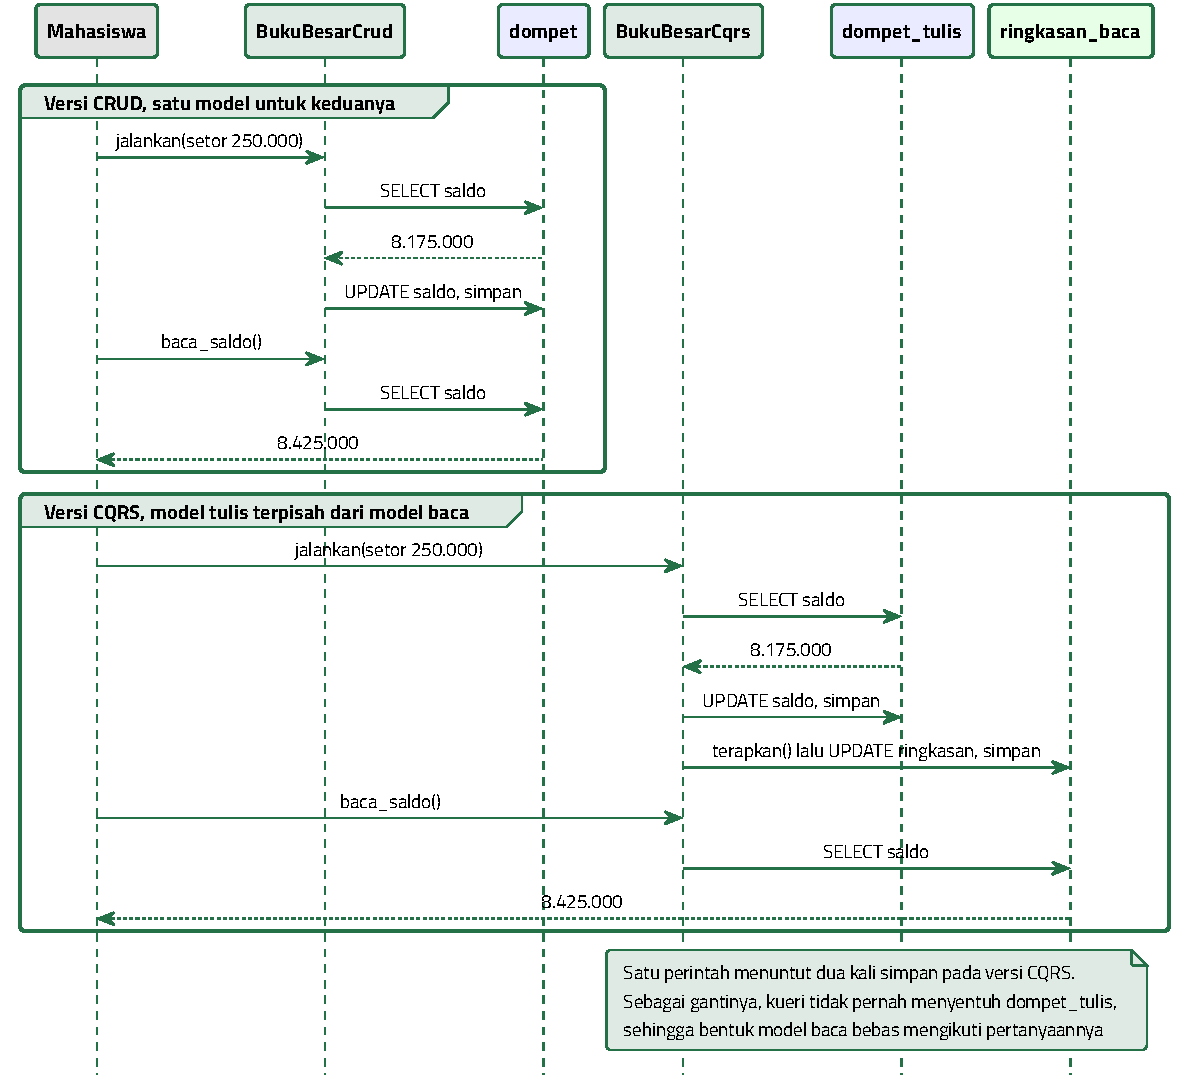
\includegraphics[width=0.94\textwidth, height=0.56\textheight,
      keepaspectratio]{sekuens-cqrs.pdf}
  \end{center}
  {\small Versi CQRS menyimpan dua kali untuk satu perintah. Sebagai gantinya,
  kuerinya tidak pernah menyentuh \texttt{dompet\_tulis}.}
\end{frame}

\begin{frame}{{\Large Menyimpan Event, Bukan Keadaan}}
  \vspace{8pt}
  \centering
  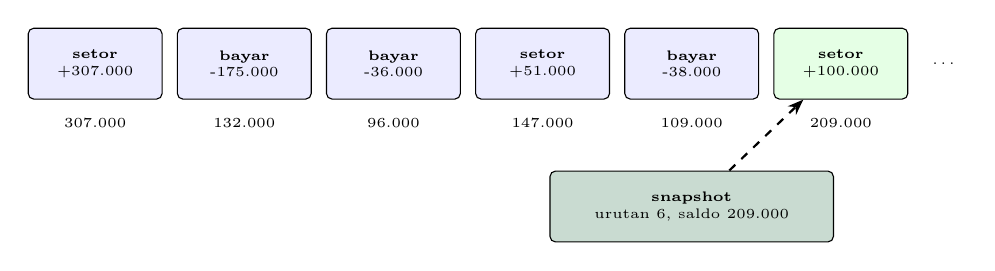
\begin{tikzpicture}[
    event/.style={draw, rounded corners=2pt, minimum width=1.7cm,
      minimum height=0.9cm, align=center, font=\tiny\bfseries},
    hasil/.style={font=\tiny, align=center},
    panah/.style={-{Stealth[length=2mm]}, thick}
  ]
    \node[event, fill=blue!8] (e1) {setor\\
      {\tiny\mdseries +307.000}};
    \node[event, fill=blue!8, right=0.18cm of e1] (e2) {bayar\\
      {\tiny\mdseries -175.000}};
    \node[event, fill=blue!8, right=0.18cm of e2] (e3) {bayar\\
      {\tiny\mdseries -36.000}};
    \node[event, fill=blue!8, right=0.18cm of e3] (e4) {setor\\
      {\tiny\mdseries +51.000}};
    \node[event, fill=blue!8, right=0.18cm of e4] (e5) {bayar\\
      {\tiny\mdseries -38.000}};
    \node[event, fill=green!10, right=0.18cm of e5] (e6) {setor\\
      {\tiny\mdseries +100.000}};
    \node[right=0.18cm of e6, font=\tiny] (lanjut) {\dots};

    \node[hasil, below=0.12cm of e1] {307.000};
    \node[hasil, below=0.12cm of e2] {132.000};
    \node[hasil, below=0.12cm of e3] {96.000};
    \node[hasil, below=0.12cm of e4] {147.000};
    \node[hasil, below=0.12cm of e5] {109.000};
    \node[hasil, below=0.12cm of e6] {209.000};

    \node[event, fill=praditagreen!25, minimum width=3.6cm,
      below=0.9cm of e5] (snap) {snapshot\\
      {\tiny\mdseries urutan 6, saldo 209.000}};
    \draw[panah, dashed] (snap) -- (e6);
  \end{tikzpicture}

  \vspace{6pt}
  {\small Lima perintah di antara pukul 08.04 dan 08.08 ditolak aturan bisnis,
  dan tidak satu pun meninggalkan baris. Log memuat yang terjadi, bukan yang
  diminta.}
\end{frame}

\begin{frame}[fragile]{{\Large Perintah Menambah Baris}}
  \vspace{4pt}
\begin{lstlisting}[style=PythonStyle]
def jalankan(self, perintah: domain.Perintah) -> int:
  """Menambah satu baris event sesudah aturan bisnisnya dipenuhi."""
  _, ringkasan = self.susun_ringkasan(perintah.pemilik)
  saldo_baru = domain.periksa_perintah(ringkasan.saldo, perintah)
  self.koneksi.execute(
    "INSERT INTO event (pemilik, jenis, nominal, waktu) "
    "VALUES (?, ?, ?, ?)",
    (perintah.pemilik, perintah.jenis, perintah.nominal, perintah.waktu),
  )
  self.koneksi.commit()
  return saldo_baru
\end{lstlisting}
  \vspace{4pt}
  {\small Tidak ada kolom saldo yang dapat dibaca langsung, sehingga saldo untuk
  memeriksa aturan bisnis disusun ulang lebih dahulu.}
\end{frame}

\begin{frame}{{\Large \textit{Class Diagram}: Empat Bagian}}
  \vspace{4pt}
  \begin{center}
    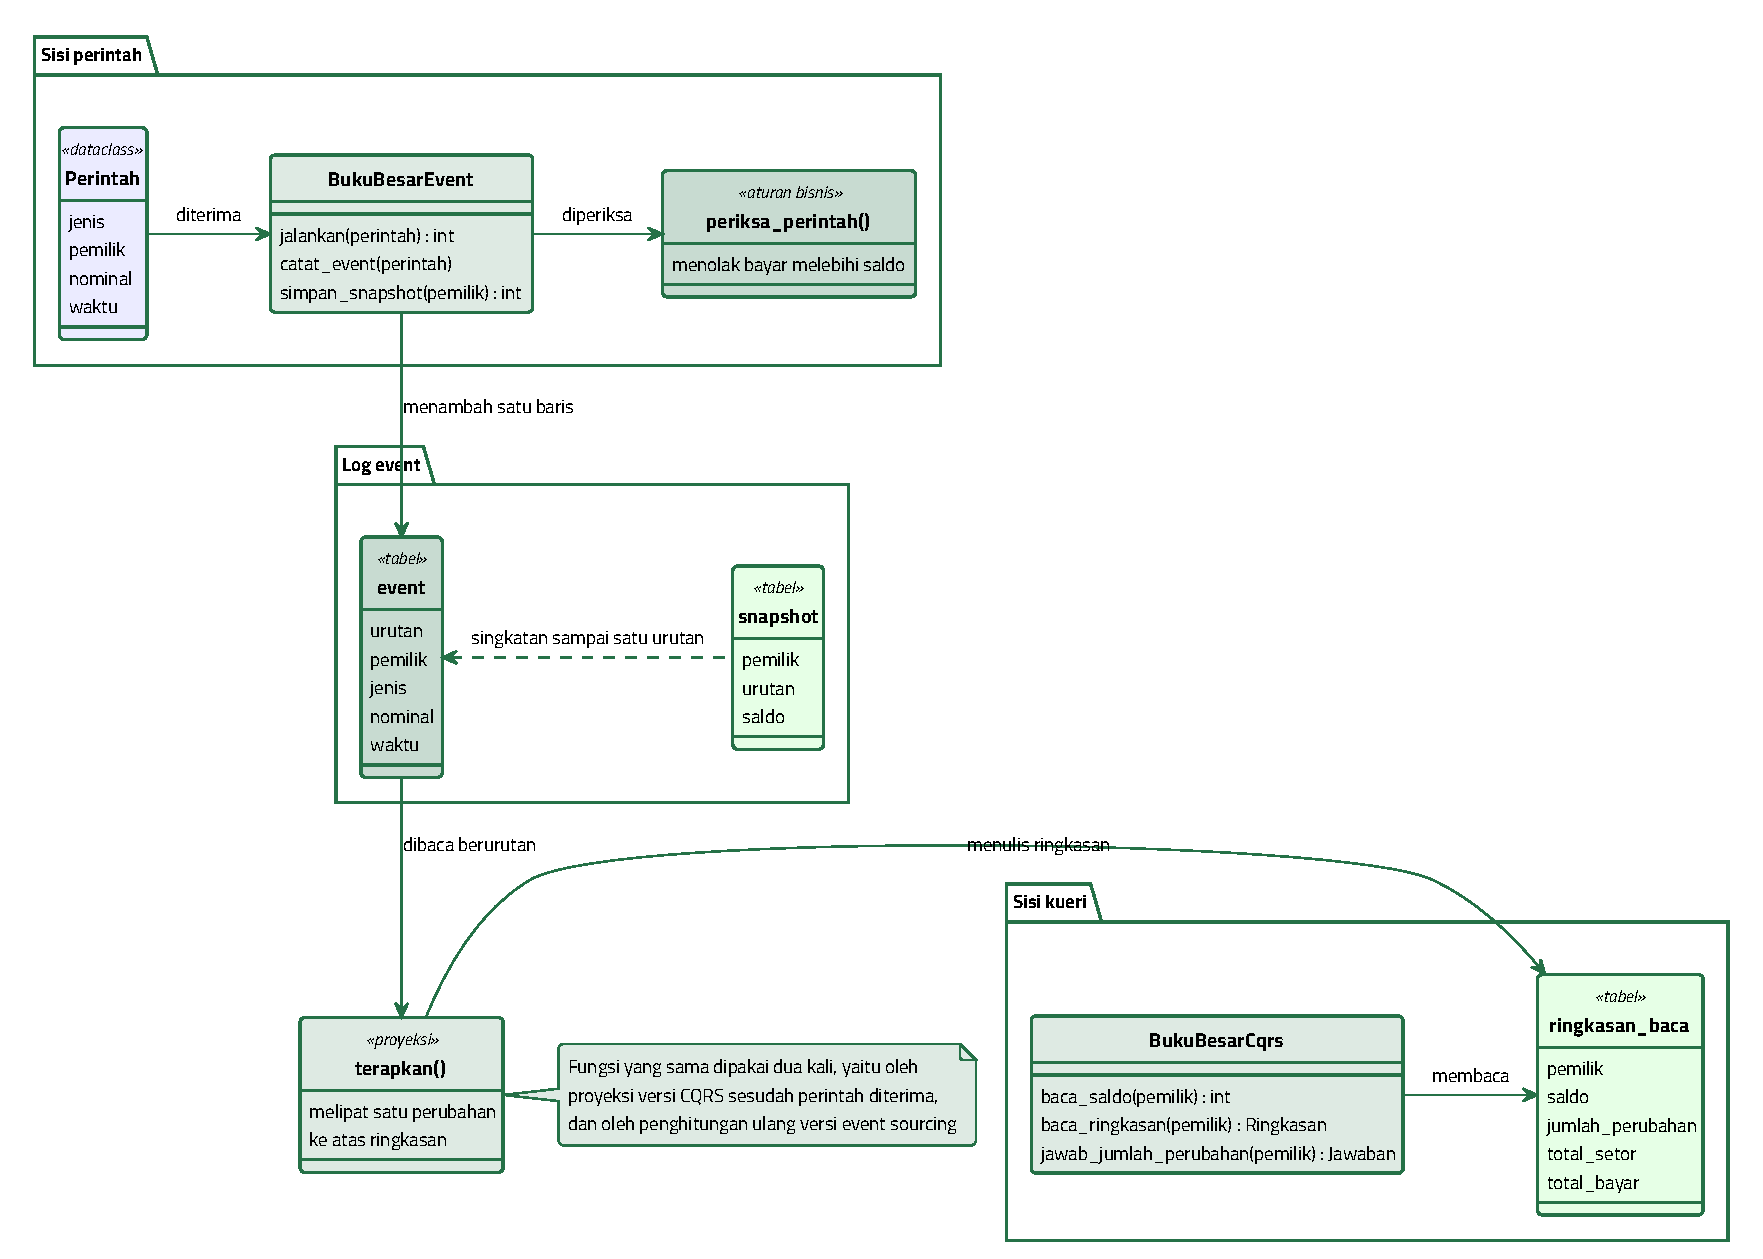
\includegraphics[width=\textwidth, height=0.76\textheight,
      keepaspectratio]{kelas-cqrs.pdf}
  \end{center}
\end{frame}

\begin{frame}{{\Large Penjelasan \textit{Class Diagram}}}
  \vspace{10pt}
  \begin{itemize}\small
    \item Panahnya satu arah, yaitu dari sisi perintah menuju
          \textit{event log}, lalu menuju model baca lewat proyeksi.
    \item \texttt{terapkan()} yang sama dipakai proyeksi versi CQRS dan
          penghitungan ulang versi \textit{event sourcing}.
    \item Snapshot hanya singkatan dari lipatan sampai satu nomor urut, dan
          boleh dibuang lalu dibentuk ulang kapan saja.
    \item Sisi kueri berhenti di model baca, sehingga tidak pernah menyentuh
          model tulis.
  \end{itemize}

  \vspace{10pt}
  {\small Ketiga versi memenuhi kontrak yang sama di \texttt{domain.py}, yaitu
  \texttt{jalankan}, \texttt{baca\_saldo}, dan \texttt{jawab\_saldo\_pada}.}
\end{frame}

\begin{frame}{{\Large Analogi: Loket dan Buku Besar}}
  \vspace{10pt}
  \begin{itemize}\small
    \item Mahasiswa yang membayar mengantre di loket keuangan, lalu petugasnya
          memeriksa tagihan dan mencatatnya.
    \item Mahasiswa yang hanya ingin tahu sisa tagihan cukup melihat portal,
          dan tidak ikut antrean itu.
    \item Portal diperbarui sesudah loket mencatat, bukan pada saat yang sama
          persis.
    \item Buku besar koperasi menulis setiap transaksi pada baris baru, dan
          saldo akhir halaman ditulis di bagian bawah halaman.
  \end{itemize}

  \vspace{10pt}
  {\small Angka di bawah halaman itulah snapshotnya. Bila diragukan, seluruh
  barisnya masih ada dan dapat dijumlah ulang.}
\end{frame}

\begin{frame}{{\Large Kasus: Pemotongan Dua Kali}}
  \vspace{8pt}
  \begin{enumerate}\small
    \item Unit keuangan menjalankan dompet mahasiswa di atas satu tabel
          keadaan.
    \item Pekerjaan pemotongan tagihan berjalan dua kali karena percobaan ulang
          yang gagal terdeteksi.
    \item Pimpinan menanyakan siapa saja yang terpotong dua kali dan berapa
          saldo mereka sebelumnya.
    \item Tabelnya hanya memuat saldo terakhir, sehingga kedua pertanyaan itu
          tidak terjawab dari sistem.
  \end{enumerate}

  \vspace{8pt}
  {\small Bukti transfer diminta dari mahasiswa satu per satu, lalu dicocokkan
  dengan tangan selama dua minggu.}
\end{frame}

\begin{frame}{{\Large Hasil: \textit{Write Cost} dan \textit{Read Cost}}}
  \vspace{6pt}
  \centering
  \small
  \begin{tabularx}{0.92\textwidth}{|X|l|l|l|}
    \hline
    \textbf{Yang diukur} & \textbf{Median} & \textbf{Persentil ke-95} & \textbf{Terbesar} \\
    \hline
    Tulis CRUD & 2,1958 ms & 2,6481 ms & 3,2731 ms \\
    \hline
    Tulis CQRS & 4,6257 ms & 5,4658 ms & 7,8009 ms \\
    \hline
    Tulis \textit{event sourcing} & 2,5998 ms & 2,9981 ms & 3,4557 ms \\
    \hline
    Baca CRUD & 0,0695 ms & 0,1249 ms & 0,1472 ms \\
    \hline
    Baca CQRS & 0,0726 ms & 0,0835 ms & 0,1047 ms \\
    \hline
    Baca \textit{event sourcing} & 0,3078 ms & 0,4598 ms & 0,5240 ms \\
    \hline
  \end{tabularx}

  \vspace{6pt}
  {\small Versi CQRS justru menulis paling lambat, sebab satu perintah menuntut
  dua kali simpan ke cakram.}
\end{frame}

\begin{frame}{{\Large Hasil: \textit{Replay Cost}}}
  \vspace{6pt}
  \centering
  \small
  \begin{tabularx}{0.92\textwidth}{|X|l|l|l|}
    \hline
    \textbf{Yang dilaporkan} & \textbf{1.000} & \textbf{10.000} & \textbf{100.000} \\
    \hline
    Median tanpa snapshot & 1,9146 ms & 17,1736 ms & 173,9364 ms \\
    \hline
    Median dengan snapshot & 0,7147 ms & 0,6083 ms & 2,9440 ms \\
    \hline
    Persentil ke-95 tanpa snapshot & 2,5361 ms & 28,0888 ms & 602,7324 ms \\
    \hline
    Snapshot mempercepat & 2,7 kali & 28,2 kali & 59,1 kali \\
    \hline
    Ukuran \textit{event log} & 92,0 KiB & 668,0 KiB & 6.720,0 KiB \\
    \hline
  \end{tabularx}

  \vspace{6pt}
  {\small Jalur tanpa snapshot tumbuh sejalan dengan panjang lognya, sedangkan
  jalur bersnapshot selalu melipat 250 event terakhir.}
\end{frame}

\begin{frame}{{\Large Hasil: Ruang dan \textit{Temporal Query}}}
  \vspace{6pt}
  \centering
  \small
  \begin{tabularx}{0.92\textwidth}{|l|l|l|X|}
    \hline
    \textbf{Versi} & \textbf{Ukuran} & \textbf{Saldo 08.30} & \textbf{Jumlah perubahan} \\
    \hline
    CRUD & 12,0 KiB & tidak terjawab & tidak terjawab \\
    \hline
    CQRS & 20,0 KiB & tidak terjawab & 95 \\
    \hline
    \textit{Event sourcing} & 668,0 KiB & 2.132.000 & 95 \\
    \hline
  \end{tabularx}

  \vspace{6pt}
  {\small Sepuluh ribu perintah, 9.995 di antaranya diterima.
  \textit{Event log}-nya 55,7 kali berkas keadaan, dan setiap event
  menghabiskan sekitar 68 bita.}
\end{frame}

\begin{frame}{{\Large \textit{Summary}}}
  \vspace{10pt}
  \begin{itemize}\small
    \item CQRS memisahkan model tulis dari model baca, dan proyeksilah yang
          menjembatani keduanya.
    \item Pemisahan itu berbayar, yaitu satu perintah menuntut dua kali simpan,
          4,6257 ms melawan 2,1958 ms.
    \item \textit{Event sourcing} menyimpan event, sehingga riwayatnya
          utuh, tetapi bacanya naik menjadi 0,3078 ms.
    \item Snapshot menekan penghitungan ulang, yaitu 59,1 kali lebih cepat pada
          seratus ribu event.
  \end{itemize}

  \vspace{10pt}
  {\small Pesan utamanya, penimpaan satu baris adalah keputusan yang memilih
  kemurahan tulis dan membuang riwayat.}
\end{frame}

\begin{frame}[fragile]{{\Large Persiapan Latihan}}
  \vspace{5pt}
\begin{lstlisting}[language=bash]
bash sources/siapkan_venv.sh
source .venv/bin/activate
cd sources/chapter10
python versi_event.py
# Event tersimpan    : 95
\end{lstlisting}

  \vspace{6pt}
  {\small Bab ini hanya memakai pustaka standar Python, termasuk
  \texttt{sqlite3}, sehingga tidak ada pemasangan tambahan.}
\end{frame}

\begin{frame}[fragile]{{\Large Latihan 1: \textit{Write Cost} dan \textit{Read Cost}}}
  \vspace{3pt}
\begin{lstlisting}[language=bash]
python ukur_latensi.py
# Saldo akhir ketiga versi : 8425000 (sama)
# Baca event lebih lambat  : 100 dari 100
\end{lstlisting}

  \vspace{3pt}
  \begin{enumerate}\small
    \item Catat keenam baris latensi beserta median, persentil ke-95, dan nilai
          terbesarnya.
    \item Hitung berapa kali \texttt{commit} dipanggil untuk satu perintah pada
          versi CQRS.
    \item Naikkan \texttt{JUMLAH\_PERINTAH} menjadi 500, lalu catat perubahan
          latensi bacanya.
  \end{enumerate}

  \vspace{3pt}
  {\small Pertanyaan: mengapa selisih pada sisi baca layak disebut ada,
  sedangkan selisih pada sisi tulis tidak?}
\end{frame}

\begin{frame}[fragile]{{\Large Latihan 2: \textit{Replay Cost}}}
  \vspace{3pt}
\begin{lstlisting}[language=bash]
python ukur_penghitungan_ulang.py
# Snapshot mempercepat : 59.1 kali
# Saldo kedua jalur    : sama
\end{lstlisting}

  \vspace{3pt}
  \begin{enumerate}\small
    \item Catat keenam baris hasilnya beserta baris \texttt{Snapshot
          mempercepat} pada setiap panjang log.
    \item Tunjukkan baris yang membuat penghitungan melewatkan event
          sebelum snapshot.
    \item Ubah \texttt{EVENT\_SESUDAH\_SNAPSHOT} menjadi 5.000, lalu catat
          perubahannya.
  \end{enumerate}

  \vspace{3pt}
  {\small Pertanyaan: mengapa persentil ke-95 jalur tanpa snapshot jauh
  melampaui mediannya pada seratus ribu event?}
\end{frame}

\begin{frame}[fragile]{{\Large Latihan 3: \textit{Temporal Query}}}
  \vspace{3pt}
\begin{lstlisting}[language=bash]
python tanya_riwayat.py
# Pertanyaan terjawab CRUD  : 0 dari 2
# Pertanyaan terjawab event : 2 dari 2
\end{lstlisting}

  \vspace{3pt}
  \begin{enumerate}\small
    \item Catat jawaban ketiga versi atas kedua pertanyaan beserta alasannya.
    \item Bandingkan jawaban versi \textit{event sourcing} dengan baris
          \texttt{pembanding}.
    \item Tambahkan satu pertanyaan ketiga, misalnya berapa setoran terbesar,
          lalu catat versi mana yang mampu menjawab.
  \end{enumerate}

  \vspace{3pt}
  {\small Pertanyaan: kapan pemisahan model dan penyimpanan event sepadan
  dengan biayanya?}
\end{frame}

\end{document}
